% Options for packages loaded elsewhere
\PassOptionsToPackage{unicode}{hyperref}
\PassOptionsToPackage{hyphens}{url}
%
\documentclass[
]{article}
\usepackage{amsmath,amssymb}
\usepackage{iftex}
\ifPDFTeX
  \usepackage[T1]{fontenc}
  \usepackage[utf8]{inputenc}
  \usepackage{textcomp} % provide euro and other symbols
\else % if luatex or xetex
  \usepackage{unicode-math} % this also loads fontspec
  \defaultfontfeatures{Scale=MatchLowercase}
  \defaultfontfeatures[\rmfamily]{Ligatures=TeX,Scale=1}
\fi
\usepackage{lmodern}
\ifPDFTeX\else
  % xetex/luatex font selection
\fi
% Use upquote if available, for straight quotes in verbatim environments
\IfFileExists{upquote.sty}{\usepackage{upquote}}{}
\IfFileExists{microtype.sty}{% use microtype if available
  \usepackage[]{microtype}
  \UseMicrotypeSet[protrusion]{basicmath} % disable protrusion for tt fonts
}{}
\makeatletter
\@ifundefined{KOMAClassName}{% if non-KOMA class
  \IfFileExists{parskip.sty}{%
    \usepackage{parskip}
  }{% else
    \setlength{\parindent}{0pt}
    \setlength{\parskip}{6pt plus 2pt minus 1pt}}
}{% if KOMA class
  \KOMAoptions{parskip=half}}
\makeatother
\usepackage{xcolor}
\usepackage[margin=1in]{geometry}
\usepackage{color}
\usepackage{fancyvrb}
\newcommand{\VerbBar}{|}
\newcommand{\VERB}{\Verb[commandchars=\\\{\}]}
\DefineVerbatimEnvironment{Highlighting}{Verbatim}{commandchars=\\\{\}}
% Add ',fontsize=\small' for more characters per line
\usepackage{framed}
\definecolor{shadecolor}{RGB}{248,248,248}
\newenvironment{Shaded}{\begin{snugshade}}{\end{snugshade}}
\newcommand{\AlertTok}[1]{\textcolor[rgb]{0.94,0.16,0.16}{#1}}
\newcommand{\AnnotationTok}[1]{\textcolor[rgb]{0.56,0.35,0.01}{\textbf{\textit{#1}}}}
\newcommand{\AttributeTok}[1]{\textcolor[rgb]{0.13,0.29,0.53}{#1}}
\newcommand{\BaseNTok}[1]{\textcolor[rgb]{0.00,0.00,0.81}{#1}}
\newcommand{\BuiltInTok}[1]{#1}
\newcommand{\CharTok}[1]{\textcolor[rgb]{0.31,0.60,0.02}{#1}}
\newcommand{\CommentTok}[1]{\textcolor[rgb]{0.56,0.35,0.01}{\textit{#1}}}
\newcommand{\CommentVarTok}[1]{\textcolor[rgb]{0.56,0.35,0.01}{\textbf{\textit{#1}}}}
\newcommand{\ConstantTok}[1]{\textcolor[rgb]{0.56,0.35,0.01}{#1}}
\newcommand{\ControlFlowTok}[1]{\textcolor[rgb]{0.13,0.29,0.53}{\textbf{#1}}}
\newcommand{\DataTypeTok}[1]{\textcolor[rgb]{0.13,0.29,0.53}{#1}}
\newcommand{\DecValTok}[1]{\textcolor[rgb]{0.00,0.00,0.81}{#1}}
\newcommand{\DocumentationTok}[1]{\textcolor[rgb]{0.56,0.35,0.01}{\textbf{\textit{#1}}}}
\newcommand{\ErrorTok}[1]{\textcolor[rgb]{0.64,0.00,0.00}{\textbf{#1}}}
\newcommand{\ExtensionTok}[1]{#1}
\newcommand{\FloatTok}[1]{\textcolor[rgb]{0.00,0.00,0.81}{#1}}
\newcommand{\FunctionTok}[1]{\textcolor[rgb]{0.13,0.29,0.53}{\textbf{#1}}}
\newcommand{\ImportTok}[1]{#1}
\newcommand{\InformationTok}[1]{\textcolor[rgb]{0.56,0.35,0.01}{\textbf{\textit{#1}}}}
\newcommand{\KeywordTok}[1]{\textcolor[rgb]{0.13,0.29,0.53}{\textbf{#1}}}
\newcommand{\NormalTok}[1]{#1}
\newcommand{\OperatorTok}[1]{\textcolor[rgb]{0.81,0.36,0.00}{\textbf{#1}}}
\newcommand{\OtherTok}[1]{\textcolor[rgb]{0.56,0.35,0.01}{#1}}
\newcommand{\PreprocessorTok}[1]{\textcolor[rgb]{0.56,0.35,0.01}{\textit{#1}}}
\newcommand{\RegionMarkerTok}[1]{#1}
\newcommand{\SpecialCharTok}[1]{\textcolor[rgb]{0.81,0.36,0.00}{\textbf{#1}}}
\newcommand{\SpecialStringTok}[1]{\textcolor[rgb]{0.31,0.60,0.02}{#1}}
\newcommand{\StringTok}[1]{\textcolor[rgb]{0.31,0.60,0.02}{#1}}
\newcommand{\VariableTok}[1]{\textcolor[rgb]{0.00,0.00,0.00}{#1}}
\newcommand{\VerbatimStringTok}[1]{\textcolor[rgb]{0.31,0.60,0.02}{#1}}
\newcommand{\WarningTok}[1]{\textcolor[rgb]{0.56,0.35,0.01}{\textbf{\textit{#1}}}}
\usepackage{longtable,booktabs,array}
\usepackage{calc} % for calculating minipage widths
% Correct order of tables after \paragraph or \subparagraph
\usepackage{etoolbox}
\makeatletter
\patchcmd\longtable{\par}{\if@noskipsec\mbox{}\fi\par}{}{}
\makeatother
% Allow footnotes in longtable head/foot
\IfFileExists{footnotehyper.sty}{\usepackage{footnotehyper}}{\usepackage{footnote}}
\makesavenoteenv{longtable}
\usepackage{graphicx}
\makeatletter
\def\maxwidth{\ifdim\Gin@nat@width>\linewidth\linewidth\else\Gin@nat@width\fi}
\def\maxheight{\ifdim\Gin@nat@height>\textheight\textheight\else\Gin@nat@height\fi}
\makeatother
% Scale images if necessary, so that they will not overflow the page
% margins by default, and it is still possible to overwrite the defaults
% using explicit options in \includegraphics[width, height, ...]{}
\setkeys{Gin}{width=\maxwidth,height=\maxheight,keepaspectratio}
% Set default figure placement to htbp
\makeatletter
\def\fps@figure{htbp}
\makeatother
\setlength{\emergencystretch}{3em} % prevent overfull lines
\providecommand{\tightlist}{%
  \setlength{\itemsep}{0pt}\setlength{\parskip}{0pt}}
\setcounter{secnumdepth}{-\maxdimen} % remove section numbering
\ifLuaTeX
  \usepackage{selnolig}  % disable illegal ligatures
\fi
\usepackage{bookmark}
\IfFileExists{xurl.sty}{\usepackage{xurl}}{} % add URL line breaks if available
\urlstyle{same}
\hypersetup{
  pdftitle={Getting started with R for statistics and bioinformatics},
  hidelinks,
  pdfcreator={LaTeX via pandoc}}

\title{Getting started with R for statistics and bioinformatics}
\author{}
\date{\vspace{-2.5em}}

\begin{document}
\maketitle

\begin{center}\rule{0.5\linewidth}{0.5pt}\end{center}

\section{Background}\label{background}

\subsubsection{\texorpdfstring{What is
\texttt{R}?}{What is R?}}\label{what-is-r}

R is a \emph{programming language}--a way for a human to tell a computer
to do things--designed specifically for analysing data, doing
statistics, and creating graphics. It is extremely popular, and
extremely useful. Users of R can create \emph{packages}, which add new
functions to R, and thanks to the existence of several thousand
publicly-available packages, R has an incredibly large range of
applications. In the field of bioinformatics, R's only main competitor
is the language Python, and knowing at least one of these is essential
to working as a bioinformatician.

\subsubsection{What makes this tutorial
different}\label{what-makes-this-tutorial-different}

There are plenty of R tutorials out there, and even some specific to
bioinformatics. Subtly, each reflects the preferences and styles of the
writer. You will eventually develop your own style, but your starting
point will greatly affect how fast you converge on a style that is
optimal for the work you're doing while reflecting your personality. And
yes, coding is a very expressive, creative activity and (in my opinion)
just as much a means of self-expression as painting or writing music.

This tutorial favours a style that: - Is \textbf{best for
bioinformatics}, where SPEED is hugely important. - Encourages
understanding of all the code at a deep level. This: - \textbf{Promotes
creativity}, by encouraging understanding of all the code at a deep
level, meaning you are free to express any idea that comes into your
head. `Black boxes' are avoided.

Because it aims to give you a deeper understanding, it spends a while on
the fundamentals. Much of what you learn in Part 1, you will not use in
everyday code because there are simpler ways to do it using more
sophisticated tools. BUT, as soon as you want to do something
\emph{special}, or \emph{creative}, or exceptionally \emph{efficient},
or \emph{new}, you will need to understand the fundamentals. Similarly,
knowing your fundamentals means you become far better at using more
advanced tools. Errors become less mysterious, results make more sense,
customising the tools becomes possible. This tutorial assumes you want
to truly learn the R language, not just use it to get one task done.

That said, the tutorial does not waste your time forcing you to learn
every single tiny feature and function in R. It focuses on examples to
help you get the key \textbf{concepts}. The best way to find and
understand specific features you want to use in your work is to find
code written by more experienced people who have done a task similar to
yours before, and learn from it---but once you've finished these
tutorials, the code you read from other people and from internet
searches will make much more sense and be much faster to absorb and
modify.

\subsubsection{Dazzling data.table and the tidyverse tyranny (do decide
to to dump
dplyr).}\label{dazzling-data.table-and-the-tidyverse-tyranny-do-decide-to-to-dump-dplyr.}

R's basic functionality can be expanded using \emph{packages}--think of
plugins for browsers or apps for a phone. Some packages fundamentally
change the way you write R code. The developers of R and R studio have
developed a collection of packages known as the \emph{tidyverse}
packages. They are immensely popular, partly because they are easy to
use, and partly because the developers of R and Rstudio have a natural
advantage in `influencing' (or \ldots{} monopolising?) the way people
code.

Unfortunately, the tidyverse way of coding is neither the optimal for
bioinformatics, nor is it the best for creativity.

The package \texttt{data.table} is a far better option. Compared to
tidyverse methods, it is much faster, saves memory, and most importantly
you can describe extremely creative and complex ideas in a very simple
way. It takes a tiny bit longer to learn the basics--maybe two full days
compared with one full day. But it is worth it. There is a special
tutorial on data.table waiting for you once you finish this one,
\href{tutorial_data_table.Rmd}{here}.

\subsubsection{How to do this tutorial}\label{how-to-do-this-tutorial}

\begin{enumerate}
\def\labelenumi{\arabic{enumi})}
\tightlist
\item
  Don't just read. Write and run all the commands yourself. If you miss
  one, others later may not run. Most importantly, \emph{play with the
  commands}. Change things around, try new things, connect ideas
  together, try to break the commands, then figure out why
  (\href{www.duckduckgo.com}{searching the web} might help).
\item
  This is about learning the fundamentals. Don't load any packages. Do
  \textbf{NOT} under any circumstances load \texttt{dplyr}, do
  \textbf{NOT} use \texttt{select}, \texttt{filter}, \texttt{arrange},
  \texttt{mutate}, or any of those silly things.
\item
  If you get stuck or you want to dig into a topic for greater
  understanding, first try R's inbuilt help functions (see below). Web
  searches can also be great, but be aware the answers vary a lot in
  quality. There is also \ldots{}
\item
  ChatGPT, which needs a short discussion \ldots{}
\end{enumerate}

\begin{itemize}
\tightlist
\item
  \textbf{Don't} \emph{use chatGPT to write code for you}, especially
  while you are learning. It generally produces awful code. In
  particular, it has been trained on code it finds on the internet, and
  it cannot distinguish good code from bad code. Since most code on the
  internet is bad, that is what it produces. It relies excessively on
  loading obscure packages to perform tasks that can easily and quickly
  be done with standard functions, it wantonly and wastefully converts
  data between different formats, makes inefficient choices, and worst
  of all, it makes it very tempting to run code you don't actually
  understand and couldn't write yourself.
\item
  \textbf{Do} \emph{use chatGPT to read the manual for you}. Once you
  already know some R, use chatGPT to remind yourself of bits you can't
  remember or haven't discovered yet. You will find yourself thinking
  ``I'm sure there is a function to do this, but I don't know what it
  is!'' That's a great time to ask chatGPT for help. Ask it for example:

  \begin{itemize}
  \tightlist
  \item
    ``What are the parameters that control the size and type of points
    in a scatterplot in base R?''
  \item
    ``How can I check whether a file exists in R?''
  \end{itemize}
\item
  \textbf{Do} \emph{use chatGPT to explain functions or code to you}.
  Excellent uses of chatGPT are questions like

  \begin{itemize}
  \tightlist
  \item
    ``Please break down this line of R code: `m
    \%\textless\textgreater\% apply( 1 , function(x)\{x/sum(x)\} )'\,''
  \item
    ``In the R code `frank(x,ties.method='dense')`, what does the
    'dense' argument mean?''
  \end{itemize}
\end{itemize}

\begin{quote}
A good rule-of-thumb is that chatGPT is something you show code
\emph{to}, not something you get code \emph{from}, especially not whole
lines or multiple lines of code.
\end{quote}

\begin{center}\rule{0.5\linewidth}{0.5pt}\end{center}

\section{Part 1: R fundamentals}\label{part-1-r-fundamentals}

\begin{longtable}[]{@{}
  >{\raggedright\arraybackslash}p{(\columnwidth - 0\tabcolsep) * \real{0.0556}}@{}}
\toprule\noalign{}
\endhead
\bottomrule\noalign{}
\endlastfoot
\#\# Starting an R session on Spartan \\
If you haven't already, start an R session by following
\href{tutorial_Rstart.html}{these} instructions. \\
\end{longtable}

\subsection{Creating and running commands in your first R
script}\label{creating-and-running-commands-in-your-first-r-script}

You will start with a screen like this \ldots{}

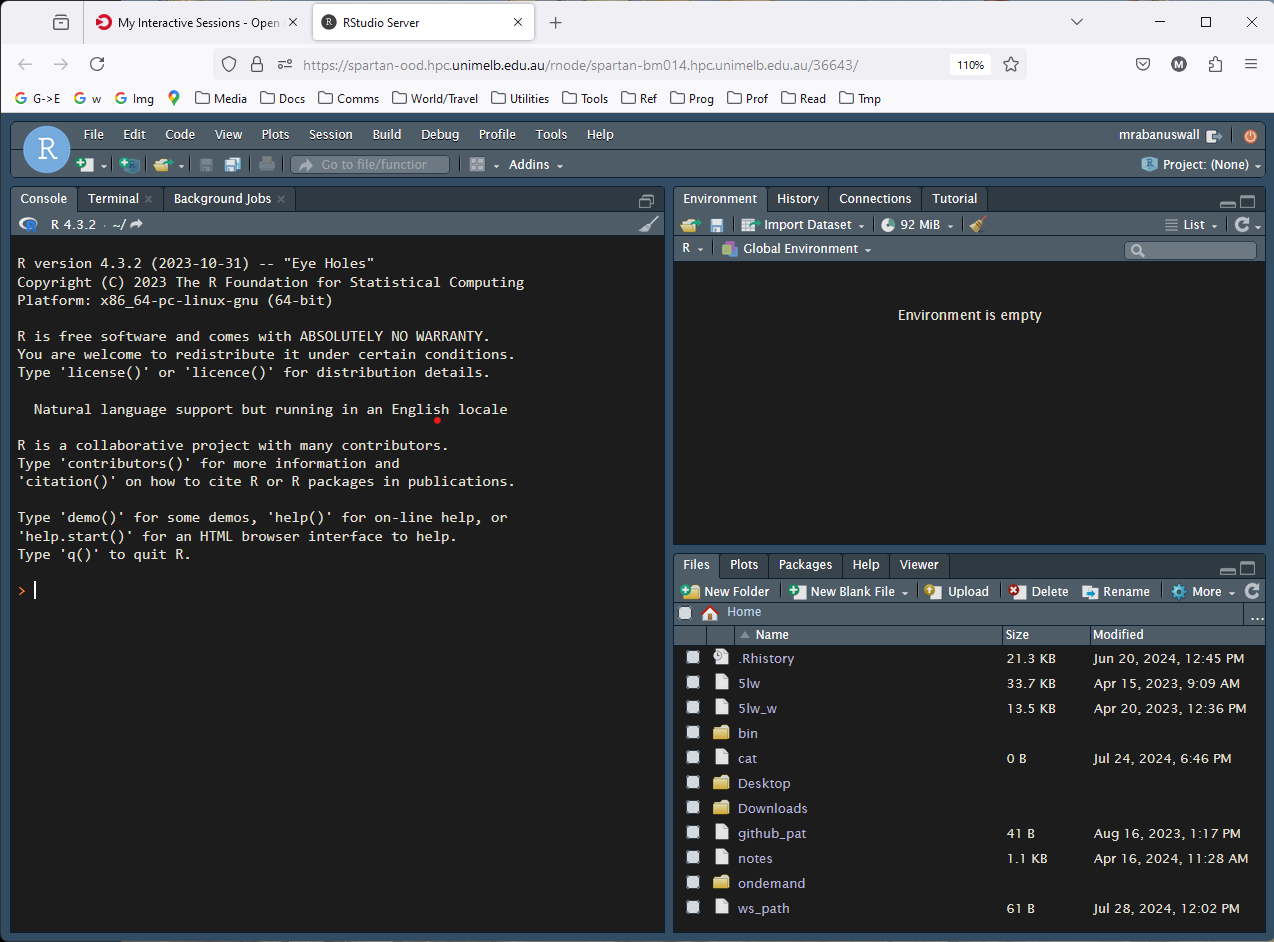
\includegraphics{images/RstudioScreen.png}

First thing, create a new \emph{script} using this button. A script is
just a text file you use to save R \emph{commands} that achieve some
task. Use \texttt{\textless{}ctrl\textgreater{}\ +\ s} so save, and name
it, say, \emph{tutorial.R}.

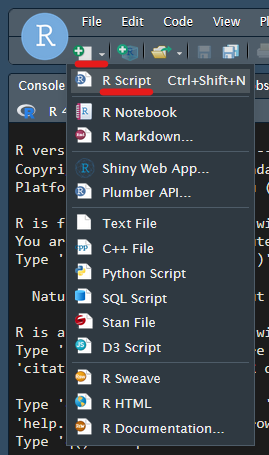
\includegraphics{images/Rscript.png}

To test things are working, type the following into the script:

\begin{Shaded}
\begin{Highlighting}[]
\NormalTok{a }\OtherTok{\textless{}{-}} \DecValTok{1}\SpecialCharTok{:}\DecValTok{10}
\FunctionTok{print}\NormalTok{(a)}
\FunctionTok{plot}\NormalTok{((}\DecValTok{1}\SpecialCharTok{:}\DecValTok{10}\NormalTok{)}\SpecialCharTok{\^{}}\DecValTok{2}\NormalTok{)}
\end{Highlighting}
\end{Shaded}

Each of these lines is a command. Let's run the first command. Highlight
the command using the mouse, then run it using
\texttt{\textless{}ctrl\textgreater{}\ +\ \textless{}return\textgreater{}}
(aka
\texttt{\textless{}ctrl\textgreater{}\ +\ \textless{}enter\textgreater{}}).

You should see this:

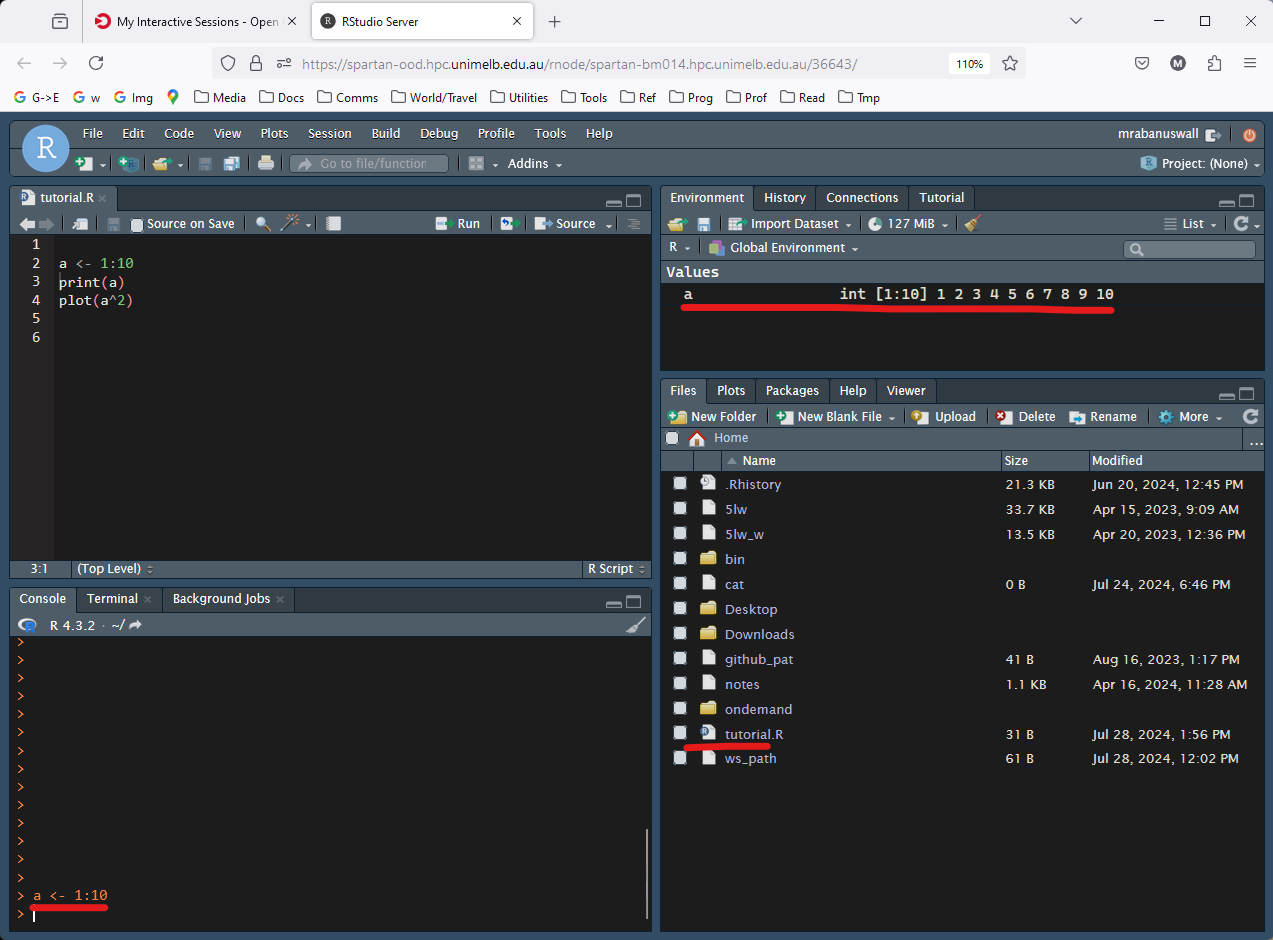
\includegraphics{images/RfirstRun.png}

Notice:

\begin{itemize}
\tightlist
\item
  The command appears in the lower left window. This is known as the
  \emph{R console}. It is analagous to the linux command line, except
  running R. It is both where commands are inputted, and where much of
  their results are outputted. You can always type commands directly
  into the console, but the trick using
  \texttt{\textless{}ctrl\textgreater{}\ +\ \textless{}return\textgreater{}}
  is a far more convenient way to work.
\item
  In the top right under the `Environment' tab, the value ``a'' is
  recorded. This will make more sense later.
\item
  In the lower right under the `Files' tab, we can see the contents of
  our home directory, including our script. This is simply a file
  browser, and is immensely useful.
\end{itemize}

Now run the second command a different way. Instead of highlighting the
command, simply place the cursor on the same line, and hit
\texttt{\textless{}ctrl\textgreater{}\ +\ \textless{}return\textgreater{}}.
Notice it sends the whole line to the console. This is the most common
way to run commands. We use the highlighting trick when we want to run
just small parts of larger commands.

\end{document}
